\begin{ZhChapter}

\chapter{實驗結果與討論}

\section{研究問題}

本章依研究流程彙整五項研究問題（Research Questions, RQs），分別評估 CT 量化特徵、三維影像模型與肺功能衍生標籤於 COPD 輔助判讀之表現。結果分析著重於模型效能、類別辨識均衡性及其臨床判讀意義。

\begin{list}{}{\setlength{\leftmargin}{4.2em}\setlength{\labelwidth}{3.4em}\setlength{\labelsep}{0.8em}\setlength{\itemsep}{0.35em}}
    \item[\textbf{RQ1：}]胸部 CT 影像擷取之量化生物標記，能否區分 COPD 正常與異常？
    \item[\textbf{RQ2：}]輸入三維 CT 之影像模型，是否能進行正常與異常分類？
    \item[\textbf{RQ3：}]三維 CT 影像模型是否能預測肺功能塌陷角度？
    \item[\textbf{RQ4：}]塌陷角度衍生之二分類與三分類標籤，是否有助於肺功能相關影像判讀？
    \item[\textbf{RQ5：}]三維 CT 影像模型能否辨識 GOLD 相關候選分級？
\end{list}

\section{實驗環境設定}

本研究實驗於本機工作站完成，硬體設備如表~\ref{tab:experiment_hardware} 所示。CT 量化生物標記分支於 Windows 環境執行，三維 CT 深度學習、塌陷角預測、GOLD 相關候選分級與 TAP-CT 相關實驗則於 Ubuntu 環境執行。兩分支之軟體環境整理如表~\ref{tab:quant_software} 與表~\ref{tab:deep_software}。

\begin{table}[htbp]
\centering
\caption{實驗硬體設備}
\label{tab:experiment_hardware}
\begingroup
\renewcommand{\arraystretch}{1.6}
\begin{tabularx}{0.95\textwidth}{|>{\centering\arraybackslash}p{0.28\textwidth}|>{\centering\arraybackslash}X|}
\hline
\textbf{項目} & \textbf{規格} \\
\hline
CPU & Intel Core i7-12700K 3.60GHz 12-Core Processor \\
\hline
GPU & NVIDIA GeForce RTX 4070 Ti SUPER \\
\hline
RAM & 32GB DDR4-3200MHz \\
\hline
Storage & 1TB NVMe SSD + 2TB SATA HDD \\
\hline
\end{tabularx}
\endgroup
\end{table}

\begin{table}[htbp]
\centering
\caption{CT 量化生物標記分支實驗環境}
\label{tab:quant_software}
\begingroup
\renewcommand{\arraystretch}{1.45}
\begin{tabularx}{0.95\textwidth}{|>{\centering\arraybackslash}p{0.28\textwidth}|>{\raggedright\arraybackslash}X|}
\hline
\textbf{項目} & \textbf{內容} \\
\hline
作業系統 & Windows 11 Pro 64-bit \\
\hline
分割與影像處理工具 & 3D Slicer、MONAI Auto3DSeg、AeroPath、SimpleITK \\
\hline
模型訓練與資料處理套件 & PyTorch、scikit-learn、NumPy、pandas \\
\hline
\end{tabularx}
\endgroup
\end{table}

\begin{table}[htbp]
\centering
\caption{三維 CT 深度學習分支實驗環境}
\label{tab:deep_software}
\begingroup
\renewcommand{\arraystretch}{1.45}
\begin{tabularx}{0.95\textwidth}{|>{\centering\arraybackslash}p{0.28\textwidth}|>{\raggedright\arraybackslash}X|}
\hline
\textbf{項目} & \textbf{內容} \\
\hline
作業系統 & Ubuntu 24.04.4 LTS (Noble Numbat)，Linux kernel 6.17.0-29-generic，x86\_64 \\
\hline
深度學習環境 & Python 3.11、PyTorch 2.8.0、CUDA 12.8、MONAI \\
\hline
醫學影像與資料處理套件 & SimpleITK、nibabel、scikit-learn、pandas、matplotlib \\
\hline
TAP-CT 相關套件 & transformers、timm、einops \\
\hline
\end{tabularx}
\endgroup
\end{table}

\section{實驗結果分析}
\subsection{RQ1 量化特徵二分類結果}

RQ1 以 12 項 CT 衍生量化生物標記作為輸入，採五折交叉驗證評估 Normal 與 Abnormal 個案之辨識能力，結果如表~\ref{tab:rq1_quant_result} 與圖~\ref{fig:rq1_quant_cm} 所示。整體 Accuracy 為 0.9259，AUC 為 0.9784，顯示量化特徵已能有效區分兩類個案。Precision 與 Specificity 皆為 1.0000，代表本實驗未將 Normal 個案誤判為 Abnormal；Sensitivity 為 0.8788，仍有 4 筆 Abnormal 個案被判為 Normal。此結果說明肺氣腫比例、肺容積、血管與氣道等特徵具有輔助判讀價值，但異常個案漏判仍是後續模型優化的主要問題。

\begin{table}[htbp]
\centering
\caption{RQ1 量化特徵二分類結果}
\label{tab:rq1_quant_result}
\begingroup
\renewcommand{\arraystretch}{1.25}
\begin{tabularx}{0.75\textwidth}{>{\raggedright\arraybackslash}X >{\centering\arraybackslash}X >{\centering\arraybackslash}X}
\hline
指標 & 整體結果 & 五折平均 \\
\hline
Accuracy & 0.9259 & \(0.9273 \pm 0.0680\) \\
Precision & 1.0000 & \(1.0000 \pm 0.0000\) \\
Sensitivity & 0.8788 & \(0.8810 \pm 0.1086\) \\
Specificity & 1.0000 & -- \\
F1-score & 0.9355 & \(0.9331 \pm 0.0626\) \\
AUC & 0.9784 & \(0.9657 \pm 0.0430\) \\
\hline
\end{tabularx}
\endgroup
\end{table}

\begin{figure}[htbp]
\centering
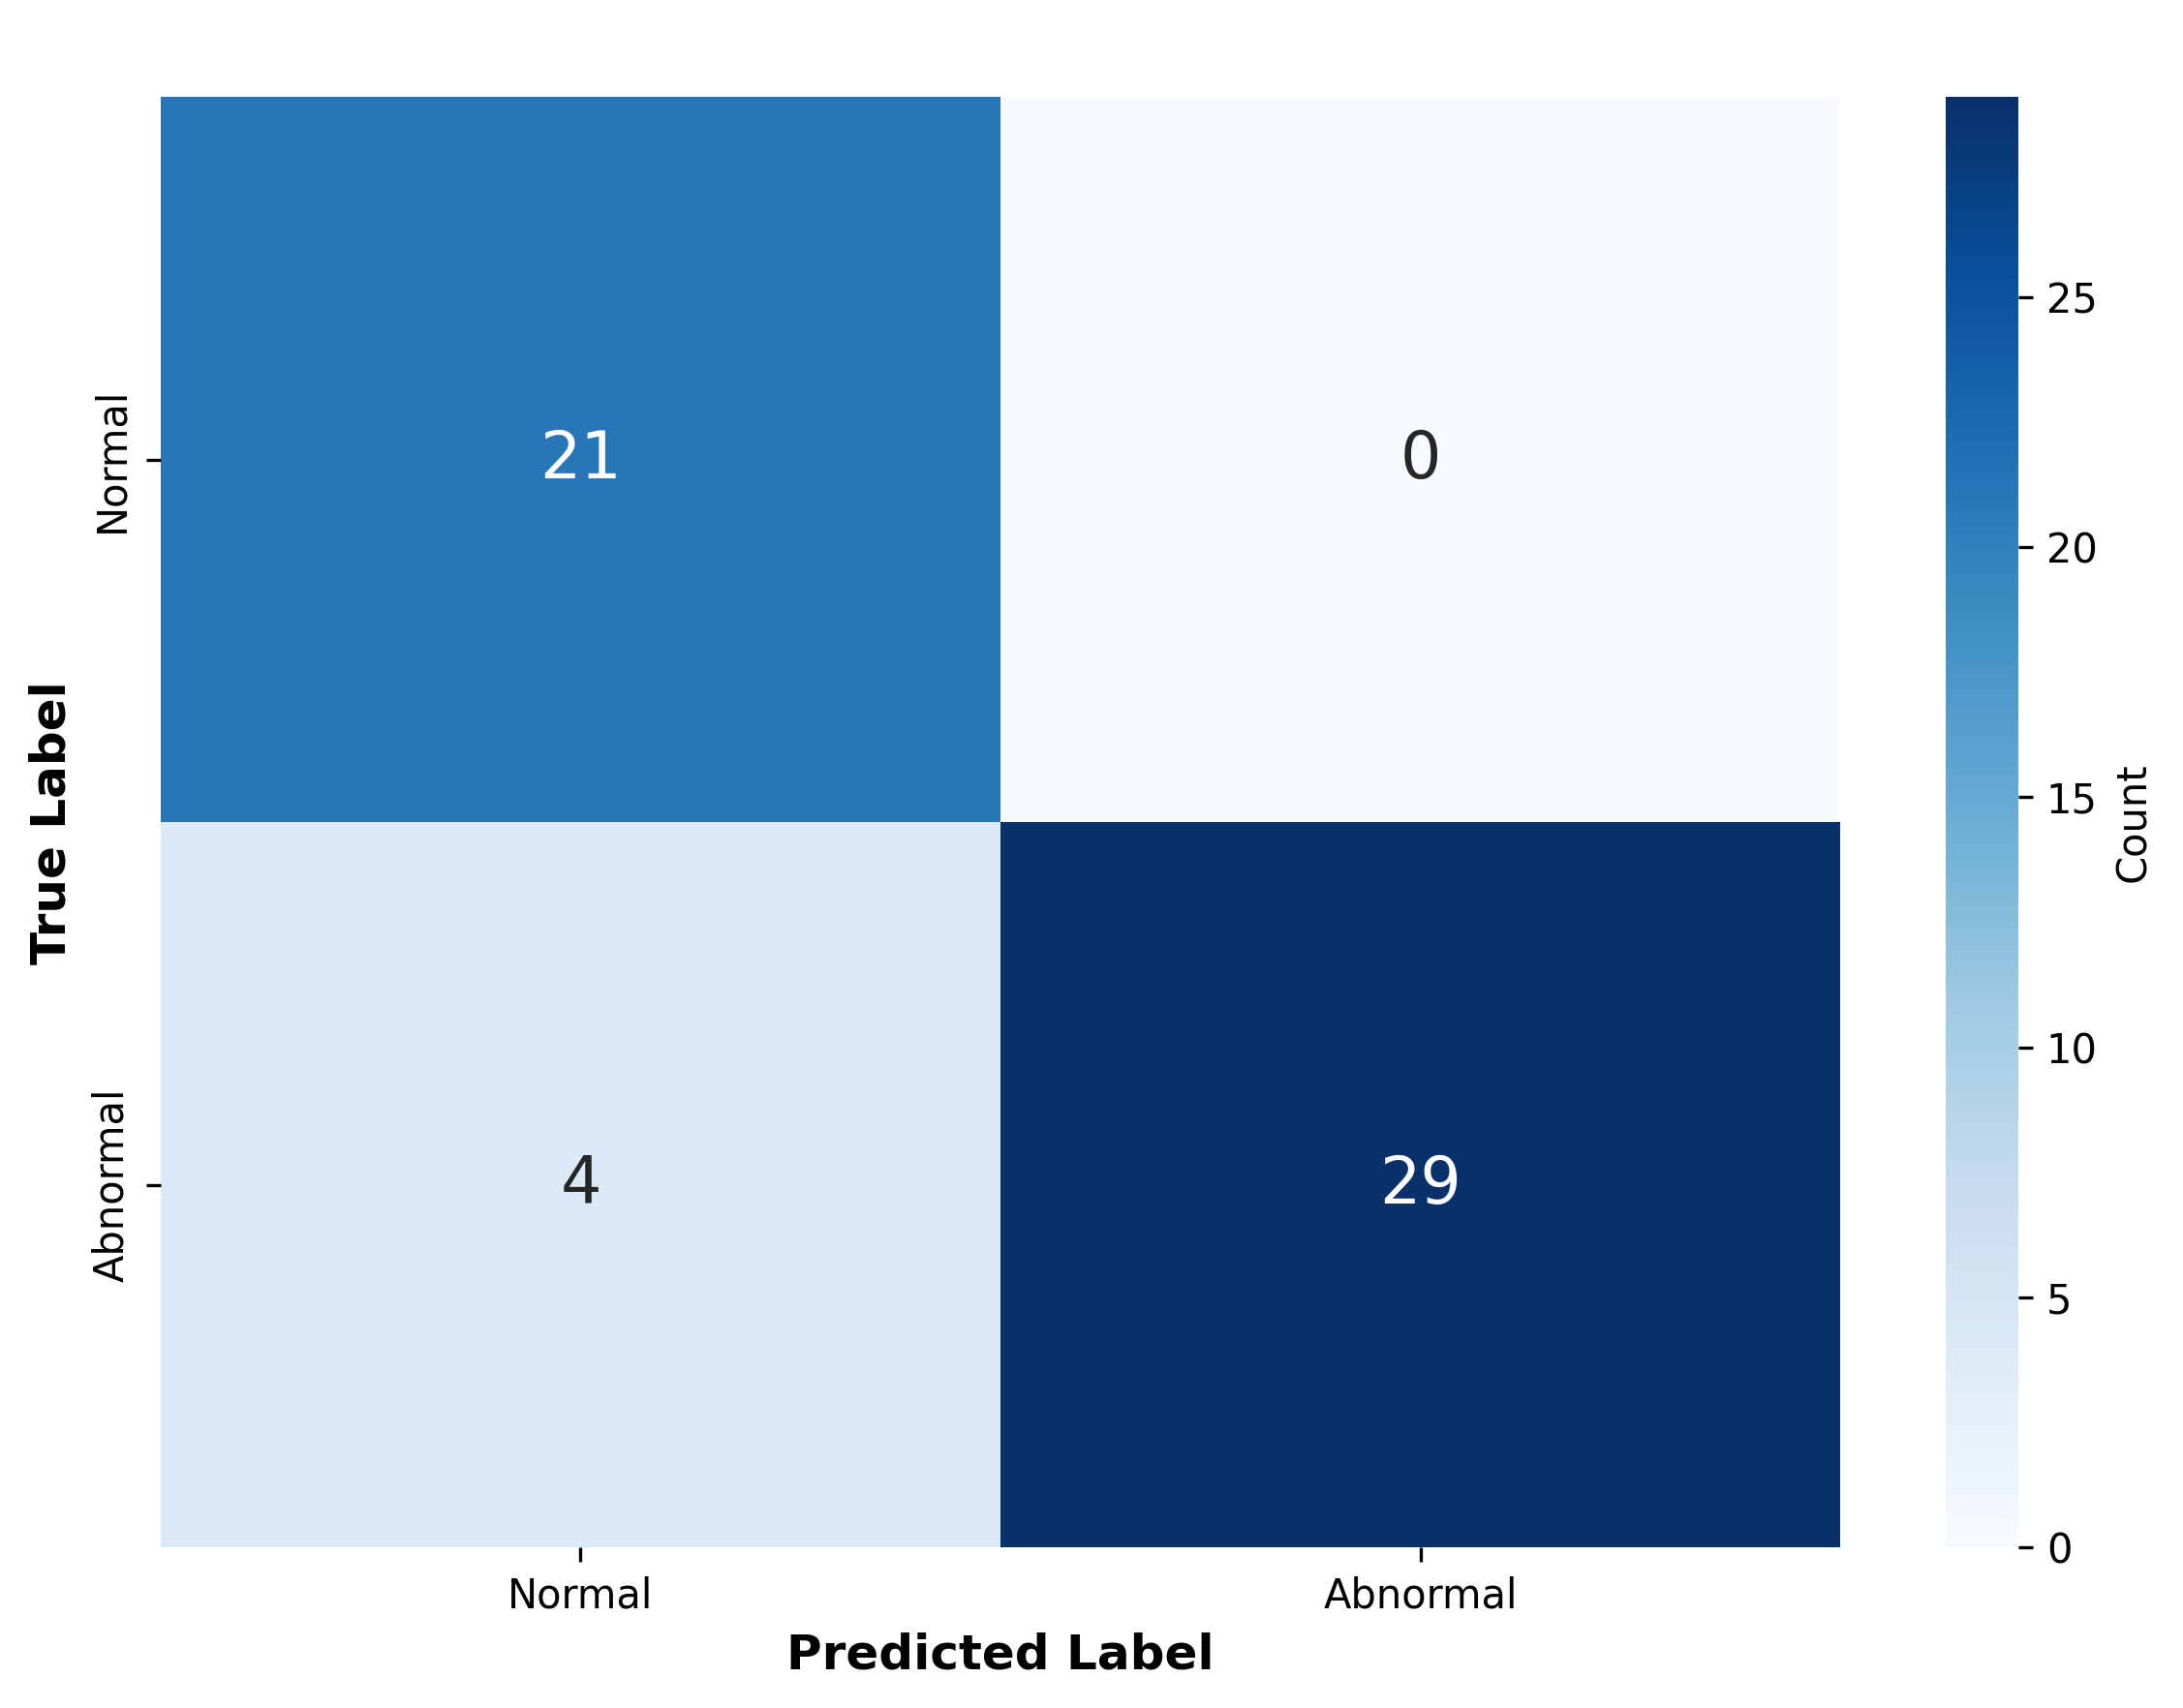
\includegraphics[width=0.80\textwidth]{figures/kfold_confusion_matrix.png}
\caption{RQ1 量化特徵二分類混淆矩陣圖}
\label{fig:rq1_quant_cm}
\end{figure}
\FloatBarrier

\subsection{RQ2 三維影像模型二分類結果}

RQ2 評估三維 CT 影像模型於 Normal/Abnormal 分類之表現。本研究採用五折平均 AUC 最高之 nnMamba e5 設定作為代表結果，各指標均以平均值與標準差呈現，如表~\ref{tab:rq2_3d_binary} 所示。

\begin{table}[htbp]
\centering
\caption{RQ2 最佳三維影像二分類結果}
\label{tab:rq2_3d_binary}
\begingroup
\renewcommand{\arraystretch}{1.25}
\begin{tabular}{l c}
\hline
指標 & 五折平均結果 \\
\hline
AUC & \(1.0000 \pm 0.0000\) \\
Accuracy & \(0.9409 \pm 0.0422\) \\
Sensitivity & \(0.9019 \pm 0.0718\) \\
Specificity & \(1.0000 \pm 0.0000\) \\
\hline
\end{tabular}
\endgroup
\end{table}

最佳三維影像模型之 AUC 為 \(1.0000 \pm 0.0000\)，Accuracy 為 \(0.9409 \pm 0.0422\)，Specificity 亦達 \(1.0000 \pm 0.0000\)。Sensitivity 為 \(0.9019 \pm 0.0718\)，顯示模型仍可能漏判部分異常個案。與 RQ1 相比，三維影像模型可直接學習三維 CT 體積資料之空間表徵，整體 Accuracy 與 AUC 略高；但其臨床應用仍需處理異常個案漏判及模型可解釋性不足的問題。
\FloatBarrier

\subsection{RQ3 三維影像角度預測結果}

RQ3 評估三維影像模型預測塌陷角連續值之能力，結果如表~\ref{tab:rq3_ac_regression} 所示。

\begin{table}[htbp]
\centering
\caption{RQ3 塌陷角連續值迴歸結果}
\label{tab:rq3_ac_regression}
\begingroup
\small
\renewcommand{\arraystretch}{1.25}
\begin{tabularx}{\textwidth}{>{\raggedright\arraybackslash}X c c c c}
\hline
模型 & MAE & RMSE & \(R^2\) & Pearson \\
\hline
Hybrid Mamba-Attention & \(15.8512 \pm 4.7756\) & 21.2647 & 0.1723 & 0.6699 \\
Mamba & \(17.1180 \pm 2.5754\) & 23.9086 & 0.0314 & 0.3413 \\
SwinUNETR & \(19.0884 \pm 2.8357\) & 24.3769 & -0.0012 & 0.1898 \\
\hline
\end{tabularx}
\endgroup
\end{table}

\begin{figure}[H]
\centering
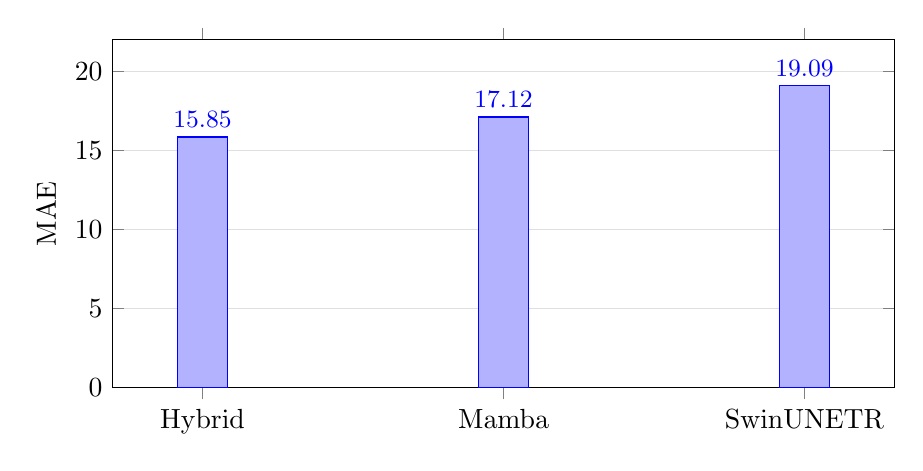
\begin{tikzpicture}
\begin{axis}[
    ybar,
    width=0.95\textwidth,
    height=6cm,
    ymin=0,
    ymax=22,
    ylabel={MAE},
    symbolic x coords={Hybrid,Mamba,SwinUNETR},
    xtick=data,
    bar width=18pt,
    enlarge x limits=0.15,
    nodes near coords,
    nodes near coords style={font=\small, /pgf/number format/fixed, /pgf/number format/precision=2},
    ymajorgrids=true,
    grid style={gray!25}
]
\addplot coordinates {(Hybrid,15.8512) (Mamba,17.1180) (SwinUNETR,19.0884)};
\end{axis}
\end{tikzpicture}
\caption{塌陷角連續值迴歸平均絕對誤差比較}
\label{fig:rq3_ac_regression}
\end{figure}

Hybrid Mamba-Attention 取得最低 MAE，平均誤差為 \(15.8512 \pm 4.7756\)，Pearson correlation 為 0.6699，皆優於其他模型。Mamba 與 SwinUNETR 之 MAE 分別為 \(17.1180 \pm 2.5754\) 與 \(19.0884 \pm 2.8357\)。結果顯示，在 Mamba 表徵後加入 attention bridge，可補充塌陷角預測所需之影像資訊；然而 \(R^2\) 仍偏低，表示單以 CT 影像精準估計連續肺功能指標仍具限制。
\FloatBarrier

\subsection{RQ4 塌陷角衍生分類結果}

RQ4 比較塌陷角衍生標籤於二分類與三分類任務中的可辨識性。以下先呈現排除 \(132^{\circ}\)--\(151^{\circ}\) 中間灰區後之 AC 二分類，再呈現保留 intermediate 類別之 AC 三分類。\texttt{baseline} 代表未加入 TAP-CT 融合或虛擬補強之原始三維 CT 設定；\texttt{pooled} 代表使用凍結之 TAP-CT 掃描嵌入，並以 ABMIL 分類頭彙整為病人層級表徵；\texttt{aug100} 與 \texttt{aug300} 則代表每類虛擬補強至 100 或 300 筆。

AC 二分類結果如表~\ref{tab:rq4_ac_binary} 所示。

\begin{table}[htbp]
\centering
\caption{RQ4 AC 二分類結果}
\label{tab:rq4_ac_binary}
\begingroup
\footnotesize
\renewcommand{\arraystretch}{1.25}
\setlength{\tabcolsep}{3pt}
\begin{tabular}{p{0.30\textwidth} p{0.14\textwidth} c c c}
\hline
模型 & 設定 & Accuracy & Macro-F1 & Bal. acc. \\
\hline
TAP-CT late fusion & aug100 & \(0.9192 \pm 0.0718\) & \(0.8763 \pm 0.1186\) & \(0.8778 \pm 0.1333\) \\
Hybrid Mamba-Attention & aug100 & \(0.8692 \pm 0.0656\) & \(0.8177 \pm 0.0761\) & \(0.8289 \pm 0.0963\) \\
Hybrid Mamba-Attention & baseline & \(0.7705 \pm 0.0323\) & \(0.4350 \pm 0.0101\) & \(0.5000 \pm 0.0000\) \\
\hline
\end{tabular}
\endgroup
\end{table}

排除中間灰區後，AC 二分類表現明顯提升。TAP-CT late fusion 搭配 aug100 取得最高 Accuracy（\(0.9192 \pm 0.0718\)）與 Macro-F1（\(0.8763 \pm 0.1186\)），相較 Hybrid Mamba-Attention baseline 之 Macro-F1 0.4350 有大幅改善。此結果指出，低角度異常傾向與高角度正常傾向兩端樣本具有較明確的影像差異。

AC 三分類結果如表~\ref{tab:rq4_ac_3class} 所示。

\begin{table}[htbp]
\centering
\caption{RQ4 AC 三分類結果}
\label{tab:rq4_ac_3class}
\begingroup
\footnotesize
\renewcommand{\arraystretch}{1.25}
\setlength{\tabcolsep}{3pt}
\begin{tabular}{p{0.30\textwidth} p{0.14\textwidth} c c c}
\hline
模型 & 設定 & Accuracy & Macro-F1 & Bal. acc. \\
\hline
TAP-CT late fusion & aug100 & \(0.8209 \pm 0.0939\) & \(0.6141 \pm 0.1403\) & \(0.6326 \pm 0.1803\) \\
TAP-CT-S-2.5D late fusion & aug100 & \(0.8352 \pm 0.0831\) & \(0.5884 \pm 0.0756\) & \(0.5933 \pm 0.0952\) \\
TAP-CT ABMIL S-3D & pooled & \(0.7132 \pm 0.0846\) & \(0.5883 \pm 0.1381\) & \(0.6400 \pm 0.2036\) \\
Hybrid Mamba-Attention & baseline & \(0.7879 \pm 0.1018\) & \(0.5861 \pm 0.1546\) & \(0.6200 \pm 0.1154\) \\
Hybrid Mamba-Attention & aug300 & \(0.7593 \pm 0.1173\) & \(0.5713 \pm 0.0748\) & \(0.6319 \pm 0.1160\) \\
\hline
\end{tabular}
\endgroup
\end{table}

AC 三分類中，TAP-CT late fusion 搭配 aug100 取得最高 Macro-F1（\(0.6141 \pm 0.1403\)），Accuracy 為 \(0.8209 \pm 0.0939\)。TAP-CT-S-2.5D late fusion 雖有最高 Accuracy（\(0.8352 \pm 0.0831\)），但 Macro-F1 較低，表示類別間辨識較不均衡。相較於二分類，三分類需額外辨識樣本數較少且界線較模糊的 intermediate 類別，因此 Macro-F1 明顯下降，顯示中間灰區會增加肺功能相關影像判讀難度。

\begin{figure}[htbp]
\centering
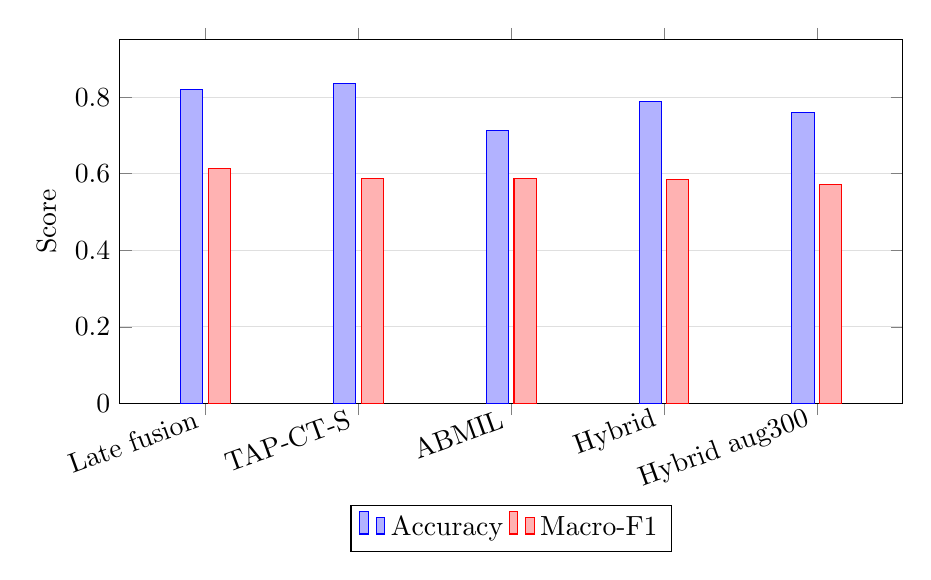
\begin{tikzpicture}
\begin{axis}[
    ybar,
    width=0.95\textwidth,
    height=6.2cm,
    ymin=0,
    ymax=0.95,
    ylabel={Score},
    symbolic x coords={Late fusion,TAP-CT-S,ABMIL,Hybrid,Hybrid aug300},
    xtick=data,
    x tick label style={rotate=20, anchor=east},
    bar width=8pt,
    enlarge x limits=0.14,
    legend style={at={(0.5,-0.28)}, anchor=north, legend columns=2},
    ymajorgrids=true,
    grid style={gray!25}
]
\addplot coordinates {(Late fusion,0.8209) (TAP-CT-S,0.8352) (ABMIL,0.7132) (Hybrid,0.7879) (Hybrid aug300,0.7593)};
\addplot coordinates {(Late fusion,0.6141) (TAP-CT-S,0.5884) (ABMIL,0.5883) (Hybrid,0.5861) (Hybrid aug300,0.5713)};
\legend{Accuracy, Macro-F1}
\end{axis}
\end{tikzpicture}
\caption{塌陷角三分類效能比較}
\label{fig:rq4_ac_3class}
\end{figure}
\FloatBarrier

\subsection{RQ5 三維影像 GOLD 相關候選分級結果}

RQ5 評估三維影像模型對 GOLD 相關候選分級之辨識能力，結果如表~\ref{tab:rq5_gold_result} 所示。由於四類樣本數不均且 GOLD 4 樣本數最少，本研究以 Macro-F1 作為主要比較指標，以降低多數類別對 Accuracy 的影響。\texttt{aug36/class} 與 \texttt{aug200/class} 分別代表於各訓練折中將類別虛擬補強至每類 36 或 200 筆，並搭配平衡取樣訓練。

\begin{table}[htbp]
\centering
\caption{RQ5 GOLD 相關候選分級結果}
\label{tab:rq5_gold_result}
\begingroup
\footnotesize
\renewcommand{\arraystretch}{1.25}
\setlength{\tabcolsep}{3pt}
\begin{tabular}{p{0.25\textwidth} p{0.16\textwidth} c c c c}
\hline
模型 & 設定 & Folds & Accuracy & Macro-F1 & Bal. acc. \\
\hline
Hybrid Mamba-Attention & \shortstack[l]{aug36\\class} & 3 & \(0.5606 \pm 0.1134\) & \(0.5323 \pm 0.0479\) & \(0.5222 \pm 0.0463\) \\
Hybrid Mamba-Attention & \shortstack[l]{基準\\F1 較佳} & 3 & \(0.5152 \pm 0.1868\) & \(0.4639 \pm 0.1645\) & \(0.5194 \pm 0.0834\) \\
Hybrid Mamba-Attention & \shortstack[l]{aug200\\class} & 3 & \(0.5606 \pm 0.0773\) & \(0.4436 \pm 0.0674\) & \(0.4611 \pm 0.0307\) \\
Hybrid Mamba-Attention & \shortstack[l]{基準\\Accuracy 較佳} & 3 & \(0.5758 \pm 0.0857\) & \(0.4355 \pm 0.0532\) & \(0.5000 \pm 0.0780\) \\
SwinUNETR & baseline & 3 & \(0.4444 \pm 0.1361\) & \(0.3144 \pm 0.1559\) & \(0.3472 \pm 0.1084\) \\
Mamba & baseline & 3 & \(0.4259 \pm 0.1458\) & \(0.3107 \pm 0.0392\) & \(0.3674 \pm 0.0606\) \\
\hline
\end{tabular}
\endgroup
\end{table}

Hybrid Mamba-Attention 搭配 aug36/class 取得最高 Macro-F1（\(0.5323 \pm 0.0479\)），Accuracy 為 \(0.5606 \pm 0.1134\)，Balanced accuracy 為 \(0.5222 \pm 0.0463\)。三個 fold 的 Accuracy 分別為 0.6818、0.5909 與 0.4091，顯示小樣本四分類仍有明顯 fold 間變異。相較於 F1 較佳之基準設定，aug36/class 將 Macro-F1 由 0.4639 提升至 0.5323；Accuracy 較佳之基準設定雖有最高 Accuracy 0.5758，但 Macro-F1 僅 0.4355，代表整體正確率較高不必然反映各類別辨識能力。aug200/class 的 Accuracy 與 aug36/class 相同，但 Macro-F1 降至 0.4436，顯示過量補強未能改善類別平均表現。

\begin{figure}[htbp]
\centering
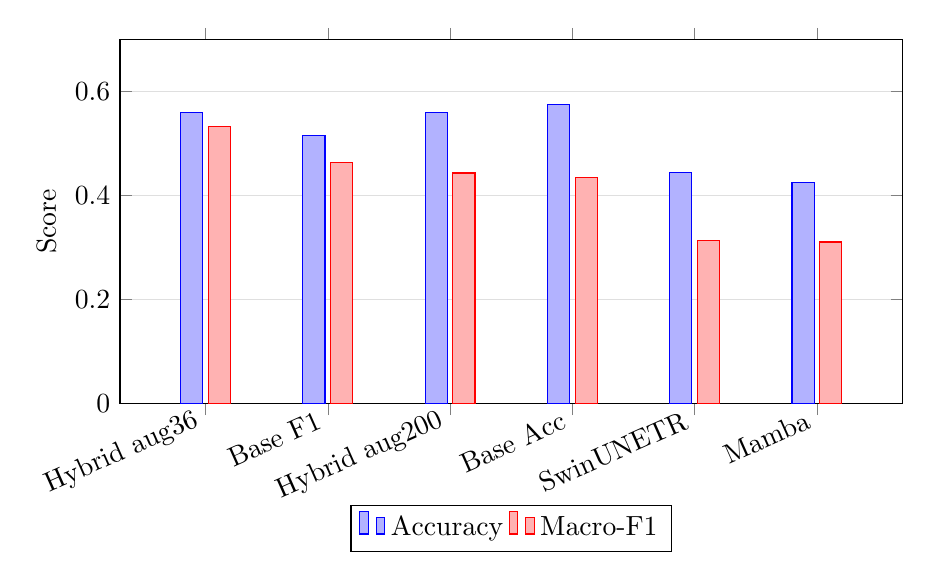
\begin{tikzpicture}
\begin{axis}[
    ybar,
    width=0.95\textwidth,
    height=6.2cm,
    ymin=0,
    ymax=0.7,
    ylabel={Score},
    symbolic x coords={Hybrid aug36,Base F1,Hybrid aug200,Base Acc,SwinUNETR,Mamba},
    xtick=data,
    x tick label style={rotate=24, anchor=east},
    bar width=8pt,
    enlarge x limits=0.14,
    legend style={at={(0.5,-0.28)}, anchor=north, legend columns=2},
    ymajorgrids=true,
    grid style={gray!25}
]
\addplot coordinates {(Hybrid aug36,0.5606) (Base F1,0.5152) (Hybrid aug200,0.5606) (Base Acc,0.5758) (SwinUNETR,0.4444) (Mamba,0.4259)};
\addplot coordinates {(Hybrid aug36,0.5323) (Base F1,0.4639) (Hybrid aug200,0.4436) (Base Acc,0.4355) (SwinUNETR,0.3144) (Mamba,0.3107)};
\legend{Accuracy, Macro-F1}
\end{axis}
\end{tikzpicture}
\caption{GOLD 候選分級分類效能比較}
\label{fig:rq5_gold_result}
\end{figure}

\end{ZhChapter}
